\subsection{Visual explanation}
The sliding window mechanism maintains a buffer buffer of a fixed length over the most recent observations from the data stream. As new data arrives, the window advances(slides) forward by a defined step size, discarding older observations while keeping elements that overlap with the previous window. The result is a data structure which allows real-time processing of continuous streams while keeping memory usage constant.\\
Figure~\ref{fig:sliding-window} shows this concept using an input consisting of the values 1 to 9, a window size of 5, and a slide step of 2. In the first iteration $n=1$, the window contains the elements ([1,2,3,4,5]). Advancing by two positions produces, the next second window ([3,4,5,6,7]). A final shift produces the third window $n=3$([5,6,7,8,9]).\\
At the implentation level the \texttt{SlidingWindow::slideWindow()} function updates the window by removing the oldest \texttt{slideStep} elements and shifting the remaining elements to the left. The positions at the end of the window are then populated with new values from the input stream.

\begin{figure}[htbp]
    \centering
    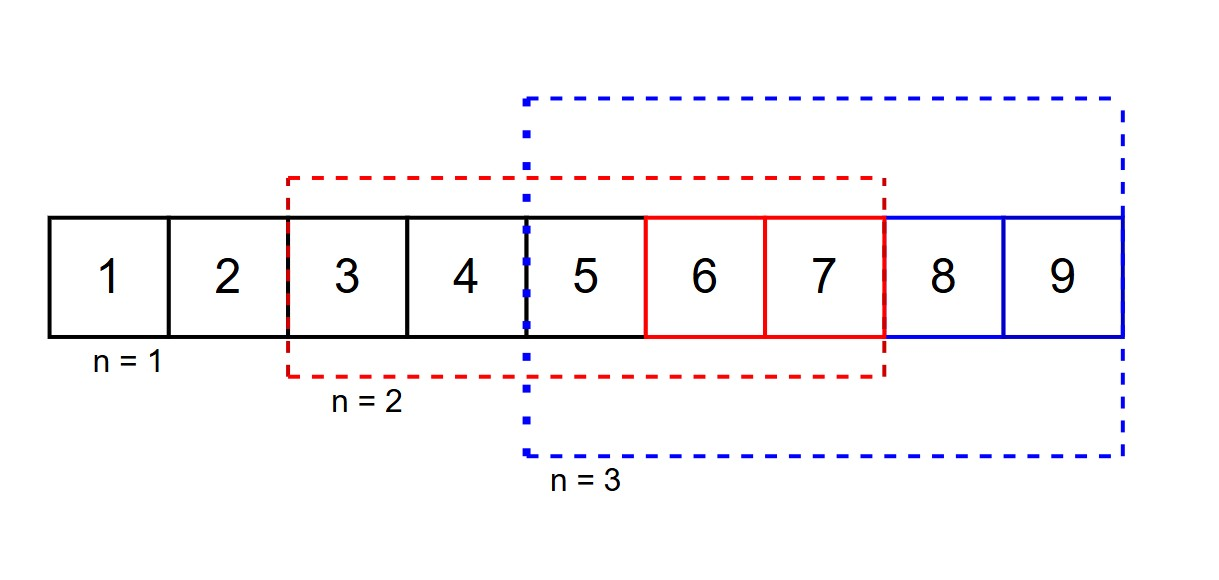
\includegraphics[width=0.35\textwidth]{figures/slidingWindowRepresentation.jpg}
    \caption{Example of a sliding window with n being the the iteration number.}
    \label{fig:sliding-window}
\end{figure}